\documentclass[compress,xcolor=table]{beamer}
% add handout to optional args for handout version

\usepackage{beamerthemesplit}
\usepackage[utf8]{inputenc}
\usepackage[german]{babel}
\usepackage{german}
\usepackage{graphicx}
\usepackage{subfigure}
\usepackage{wrapfig}
\usepackage{epsfig}
\usepackage{tabularx}
\usepackage{latexsym}
\usepackage{url}
\usepackage{tikz}
\usepackage{multimedia}
\usepackage{xcolor}
\usepackage{eso-pic}
\usepackage{color}
\usepackage{type1cm}
\usepackage{listings}
\usepackage{verbatim}
\usepackage{colortbl}
\usepackage{psfrag}
\usepackage{xifthen}
\usepackage[absolute,overlay]{textpos}
\usepackage{palatino}
\usepackage{appendixnumberbeamer}

%% Mulberry Color for highlighting
\definecolor{Mulberry}{cmyk}{0.34,0.90,0,0.02}
\definecolor{Lavender}{cmyk}{0,0.48,0,0}
\definecolor{Melon}{cmyk}{0,0.46,0.50,0}
\definecolor{Peach}{cmyk}{0,0.50,0.70,0}
\definecolor{RedOrange}{cmyk}{0,0.77,0.87,0}
\definecolor{BrickRed}{cmyk}{0,0.89,0.94,0.28}
\definecolor{Mahogany}{cmyk}{0,0.85,0.87,0.35}
\definecolor{BurntOrange}{cmyk}{0,0.51,1,0}
\definecolor{BitterSweet}{cmyk}{0,0.75,1,0.24}
\definecolor{FawkesRed}{rgb}{0.53,0,0}
\definecolor{RosBlue}{rgb}{0.19,0.25,0.38}


\mode<presentation>
{
  \usetheme{FawkesSimple}

  % to hide nav bar uncomment this line
  \setbeamertemplate{navigation symbols}{}

  %\setbeamercovered{transparent}
  \setbeamercovered{%
    again covered={\opaqueness<1->{40}}
  }
}

% Usage notes for handout version:
% Compile the beamer version immediately before you build the handout version,
% otherwise page numbers etc. will be wrong! The .aux files are *not* updated
% in handout mode, see PGF Manual for details why this is necessary.
% Comment out below one of the two pgfuselayout lines for either 2 or 4 slides
% per page. To have a very light grey background uncomment the background canvas
% color line. The logical page options are used to draw borders around each
% slide.
\mode<handout>
{
  \usetheme{FawkesSimple}

  % to hide nav bar uncomment this line
  \setbeamertemplate{navigation symbols}{}

  %\setbeamercovered{transparent}
  \setbeamercovered{%
    again covered={\opaqueness<1->{40}}
  }

  % Very slight grey background, can be used instead of borders
  %\setbeamercolor{background canvas}{bg=black!5}

  \usepackage{pgfpages}
  %% \pgfpagesuselayout{4 on 1}[a4paper,border shrink=5mm,landscape]
  \pgfpagesuselayout{2 on 1}[a4paper,border shrink=5mm]

  \pgfpageslogicalpageoptions{1}{border code=\pgfstroke}
  \pgfpageslogicalpageoptions{2}{border code=\pgfstroke}
  \pgfpageslogicalpageoptions{3}{border code=\pgfstroke}
  \pgfpageslogicalpageoptions{4}{border code=\pgfstroke}
  \nofiles
}


% Declare layers
\pgfdeclarelayer{background}
\pgfsetlayers{background,main} 

% Load PGF libraries
\usetikzlibrary{patterns}
\usetikzlibrary{arrows}
\usetikzlibrary{topaths}
\usetikzlibrary{snakes}
\usetikzlibrary{calc}
\usetikzlibrary{positioning}
\usetikzlibrary{shadows}
\usetikzlibrary{shapes.multipart}


% set lengths for textpos package
\setlength{\TPHorizModule}{10mm}
\setlength{\TPVertModule}{\TPHorizModule}
\textblockorigin{8mm}{16mm} % start everything near the top-left corner
\setbeamercolor{textblock color}{fg=blue!50,bg=white}

\urlstyle{sf}
\urldef{\projecturl}\url{}

%\pgfdeclareimage[width=4cm]{logo-big}{syslife/logo_big}

\institute{%
  %\vspace{1cm}
  \begin{minipage}{\textwidth}\centering
  
\includegraphics[height=0.6cm]{images/rwth-logo}
  \end{minipage}

  \bigskip

  \begin{minipage}{\textwidth}\centering
  \textcolor{FawkesBrown}
  \projecturl
  \end{minipage}
  %\vspace{-1.5cm}
    %  \end{column}
    %\end{columns}
  %\end{minipage}
}


%\titlegraphic{\pgfuseimage{logo-big}}

% \AtBeginPart{\frame{\partpage}}

%numbers=left, numberstyle=\tiny, stepnumber=2, numbersep=5pt
\lstset{language=[GNU]C++,
        basicstyle=\small,
        escapeinside={/*(*/}{/*)*/},
        breaklines=true,
        showstringspaces=false
        }

\lstdefinelanguage{JavaScript}{
  keywords={typeof, new, true, false, catch, function, return, null, catch, switch, var, if, in, while, do, else, case, break},
  keywordstyle=\color{blue}\bfseries,
  ndkeywords={class, export, boolean, throw, implements, import}, %, this
  ndkeywordstyle=\color{darkgray}\bfseries,
  identifierstyle=\color{black},
  sensitive=false,
  comment=[l]{//},
  morecomment=[s]{/*}{*/},
  commentstyle=\color{purple}\ttfamily,
  stringstyle=\color{red}\ttfamily,
  morestring=[b]',
  morestring=[b]"
}

\lstdefinestyle{JSON}
{
  language=JavaScript,
  morekeywords={interface,field,message,comment},
  basicstyle=\footnotesize\ttfamily\vspace{0.2cm},
  breaklines=true,
  showstringspaces=false,
  %keywordstyle=\bfseries,
  keywordstyle=\color{Mulberry},
  frame=lines,
  belowcaptionskip=8pt,
  emphstyle=\itshape,
  numbers=left,
  stepnumber=1,
  backgroundcolor=\color{blue!10},
  rulecolor=\color{blue!50},
  fillcolor=\color{blue!20},
  framexleftmargin=16pt,
  xleftmargin=16pt,
  %stringstyle=\color{BitterSweet},
  stringstyle=\color{BrickRed},
  commentstyle=\color{BrickRed},
  escapechar=\%
  % emph={getup, servo, depends_skills},
  %emphstyle=\underbar,
  %numbers=left,
  %stepnumber=1,
  %%stringstyle=\ttfamily, % typewriter type for strings
}

\lstdefinestyle{SmallJSON}{
  style=JSON,
  basicstyle=\ttfamily\footnotesize,
  numbersep=6pt,
}
\lstdefinestyle{ReallySmallJSON}{
  style=JSON,
  basicstyle=\ttfamily\tiny,
  numbersep=5pt,
}


% Listings stuff
\lstdefinelanguage{Lua}
{
  morekeywords={and,break,do,else,elseif,end,false,for,function,
                if,in,local,nil,not,or,repeat,return,then,true,until,while},
  sensitive=true,
  morecomment=[l]{--},
  morecomment=[s]{--[[}{--]]},
  morestring=[b]{"},
  morestring=[s]{[==[}{]==]},
}

% default style
\lstdefinestyle{Lua}
{
  language=Lua,
  basicstyle=\ttfamily,
  breaklines=true,
  showstringspaces=false,
  %keywordstyle=\bfseries,
  keywordstyle=\color{Mulberry},
  %frame=lines,
  %belowcaptionskip=8pt,
  emphstyle=\itshape,
  %numbers=left,
  stepnumber=1,
  %backgroundcolor=\color{blue!10},
  rulecolor=\color{blue!50},
  fillcolor=\color{blue!20},
  %framexleftmargin=18pt,
  %xleftmargin=18pt,
  stringstyle=\color{BitterSweet},
  %stringstyle=\color{BrickRed},
  commentstyle=\color{BrickRed},
  escapechar=\%
  % emph={getup, servo, depends_skills},
  %emphstyle=\underbar,
  %numbers=left,
  %stepnumber=1,
  %%stringstyle=\ttfamily, % typewriter type for strings
}
\lstdefinestyle{SmallLua}{
  style=Lua,
  basicstyle=\ttfamily\footnotesize,
  numbersep=6pt,
}
\lstdefinestyle{ReallySmallLua}{
  style=Lua,
  basicstyle=\ttfamily\tiny,
  numbersep=5pt,
}

% Default is Lua
\lstset{style=Lua}


% Hyphenation of words with hyphen
\def\hyph{-\penalty0\hskip0pt\relax}


% define an anchor in the frame
\newcommand{\tikzref}[1]{%
  \tikz[remember picture]{%
    \coordinate (#1) at (0,0.5ex);%
  }%
}%


%%% Local Variables: 
%%% mode: latex
%%% TeX-master: "iros2012-robodb"
%%% End: 


\newcommand{\backupbegin}{
   \newcounter{finalframe}
   \setcounter{finalframe}{\value{framenumber}}
}
\newcommand{\backupend}{
   \setcounter{framenumber}{\value{finalframe}}
}

% define vector/matrix helpers
\newcommand*\colvec[3][]{
    \begin{pmatrix}\ifx\relax#1\relax\else#1\\\fi#2\\#3\end{pmatrix}
}
\newcommand{\mattwo}[4]{\begin{pmatrix} #1 & #2 \\ #3 & #4\end{pmatrix}}


\title[Combining 3D Shape, Color, and Motion for Robust Anytime Tracking]{Combining 3D Shape, Color, and Motion\\ for Robust Anytime Tracking\\ \small{Paper by Held, Levinson, Thrun, and Savarese~\cite{paper}}}
\author[Zwilling]{%
  Frederik Zwilling\\
  \bigskip
  {\scriptsize Seminar Current Topics in Computer Vision and Machine Learning\\ RWTH Aachen University}
}

\date[\today @ Seminar CVML]{\today -- Seminar Current Topics in Computer Vision and Machine Learning}

\begin{document}

\frame[plain]{\titlepage}
\addtocounter{framenumber}{-1}

\begin{frame}
  \frametitle{Agenda}
  \tableofcontents[hideallsubsections]
\end{frame}

\section{Motivation}

\begin{frame}
  \frametitle{Tracking for Autonomous Cars}
  
  \begin{columns}
  \begin{column}{0.6\textwidth}
  \begin{description}[]
  \item[Chances] \hfill \\
  \begin{itemize}
  \item Free use of driving time
  \item Help disabled persons
  \item Computers do not get\\tired or drunk
  \item Faster reaction time
  \item[$\Rightarrow$] Safe 26k lifes per year in EU
  \end{itemize}
  \end{description}
  \end{column}
  \begin{column}{0.4\textwidth}
  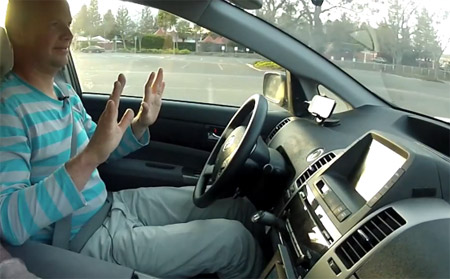
\includegraphics[width=\textwidth]{images/auto.jpg}
  \end{column}
  \end{columns}
  \pause
  \bigskip
  \begin{columns}
  \begin{column}{0.6\textwidth}
  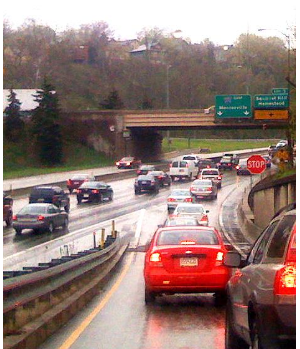
\includegraphics[height=0.35\textheight]{images/highway}
  \hspace{0.01cm}
  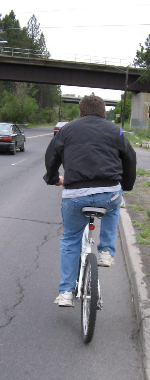
\includegraphics[height=0.35\textheight]{images/cycle}
  \hspace{0.01cm}
  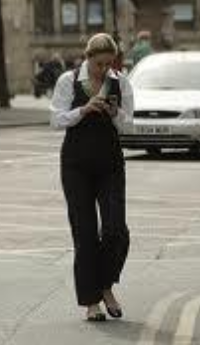
\includegraphics[height=0.35\textheight]{images/pedestrian}
  \end{column}
  \begin{column}{0.5\textwidth}
  \begin{description}[]
  \item[Challenges] \hfill \\
  \begin{itemize}
  \item Precise tracking
  \item Robustness
  \item Occlusion
  \item Real time
  \end{itemize}
  \end{description}
  \end{column}
  \end{columns}
\end{frame}

\begin{frame}
  \frametitle{Tracking for Autonomous Cars}
  \begin{description}[]
  \item[Subtasks of Tracking] \hfill \\
  \begin{itemize}
  \item Segment sensor data into objects
  \item Associate objects in successive frames
  \item Position and velocity estimation
  \item Object and trajectory classification
  \end{itemize}
  \end{description}
  \pause
  \begin{block}{Topic of this presentation}
    Position and velocity estimation
  \end{block}
\end{frame}

\begin{frame}
  \frametitle{Given Sensor Data}

  \begin{columns}
  \begin{column}{0.6\textwidth}
  \begin{description}[]
  \item[Sensor] \hfill \\
  \begin{itemize}
  \item Dense 3D laser sensor
  \item Generates point cloud
  \item Additional panorama image
  \item Similar to stereo cameras\\
        but more precise and expensive
  \end{itemize}
  \pause
  \item[Given for us] \hfill \\
  \begin{itemize}
  \item Point clouds of detected objects
  \item Association between frames already done
  \end{itemize}
  \end{description}
  \end{column}
  \onslide<1->
  \begin{column}{0.4\textwidth}
  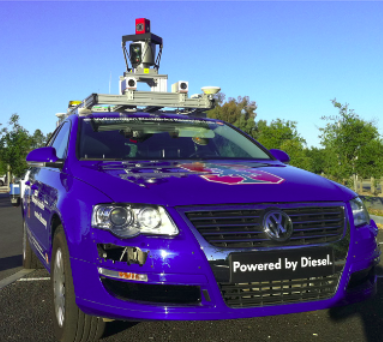
\includegraphics[width=\textwidth]{../img/lidar}\\
\bigskip
  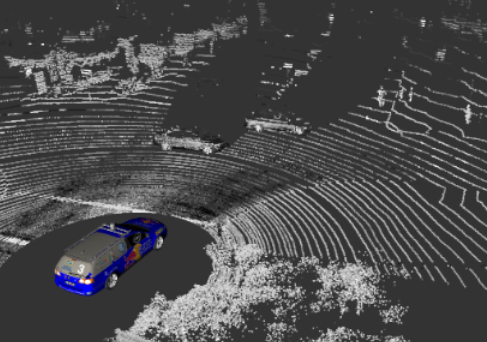
\includegraphics[width=\textwidth]{../img/lidar-data}
  \end{column}
  \end{columns}
\end{frame}

\begin{frame}
  \frametitle{Teaser Paper Ideas}
  \begin{description}[]
  \item[How to find a precise alignment?] \hfill \\
  \begin{itemize}
  \item Utilize whole object shape
  \item Additional cues from color
  \item Use motion model
  \end{itemize}
  \pause
  \item[How to search the state space fast?] \hfill \\
  \begin{itemize}
  \item Histogram with coarse initial resolution
  \item Refine resolution important areas
  \item Consider resolution in the probabilistic model
  \end{itemize}
  \end{description}
\end{frame}


\section{Baseline Methods}
\begin{frame}
  \frametitle{Baseline Methods}
  \begin{tikzpicture}[thick, every node/.style={font=\footnotesize}]
    \only<1>{
    \node (program) [outer sep=0,inner sep=0,anchor=south west]
    at (0,0)
    {
    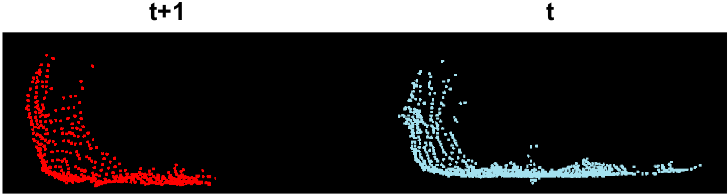
\includegraphics[width=\textwidth,height=0.25\textwidth]{images/point-clouds}};}
    \only<2>{
    \node (program) [outer sep=0,inner sep=0,anchor=south west]
    at (0,0)
    {
    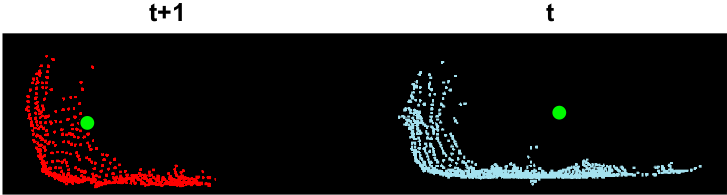
\includegraphics[width=\textwidth,height=0.25\textwidth]{images/centroid}};}
    \only<3>{
    \node (program) [outer sep=0,inner sep=0,anchor=south west]
    at (0,0)
    {
    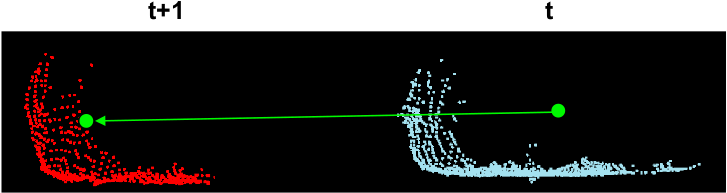
\includegraphics[width=\textwidth,height=0.25\textwidth]{images/centroid-alignment}};}
    \only<4->{
    \node (program) [outer sep=0,inner sep=0,anchor=south west]
    at (0,0)
    {
    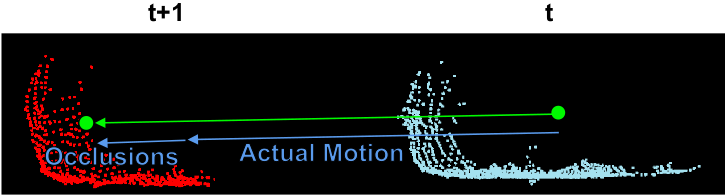
\includegraphics[width=\textwidth,height=0.25\textwidth]{images/kalman-error}};}
    \node (descx) at (10.6,-0.25)
    {\tiny \cite{held-website}};
    \onslide<1->
  \end{tikzpicture}
  
  \begin{description}[]
  \item[Kalman Filter] \hfill \\
  \begin{itemize}
  \onslide<2->{\item Aligns centroids}
  \onslide<4->{\item Problems with occlusion}
  \onslide<5->{\item Robustness through motion model}
  \onslide<6->{\item Very fast}
  \end{itemize}
  \end{description}
\end{frame}

\begin{frame}
  \frametitle{Baseline Methods}
  
  \begin{description}[]
  \item[Iterative Clostest Point (ICP)] \hfill \\
  \begin{itemize}
  \item Iterative hill climbing approach
  \item Minimizes quadratic distance of closest points
  \item Uses whole point cloud
  \pause
  \item Depends on good initialization
  \item Problem: local optima\\
  \begin{tikzpicture}[thick, every node/.style={font=\footnotesize}]
    \only<1-2>{
    \node (program) [outer sep=0,inner sep=0,anchor=south west]
    at (0,0)
    {
    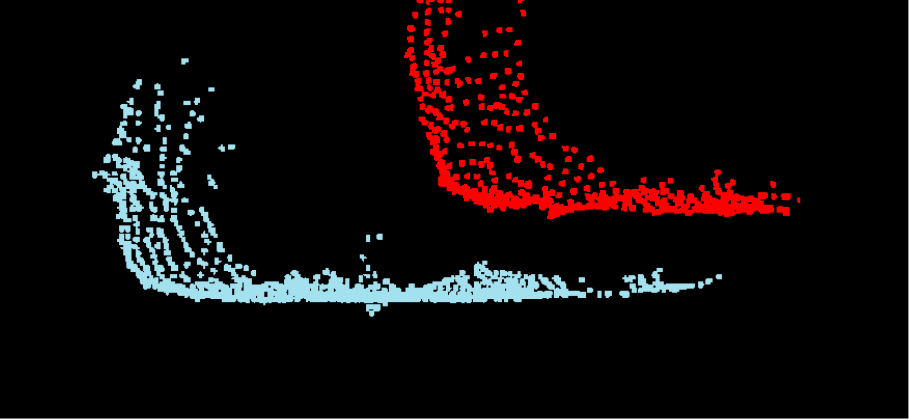
\includegraphics[height=0.25\textwidth]{images/icp-init}};}
    \only<3>{
    \node (program) [outer sep=0,inner sep=0,anchor=south west]
    at (0,0)
    {
    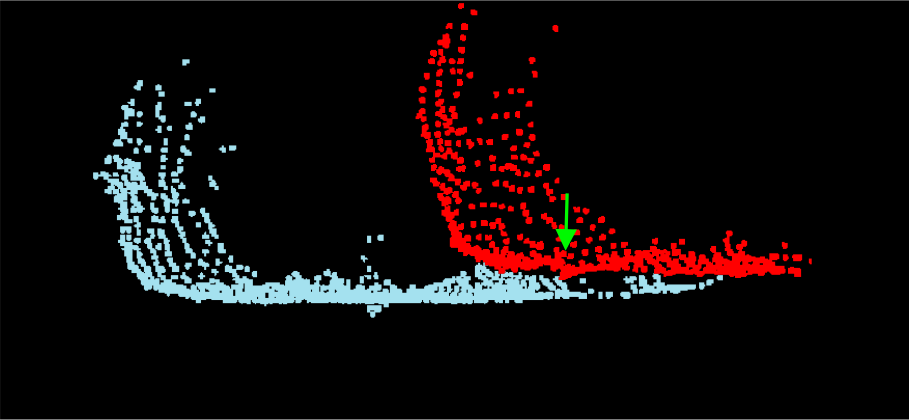
\includegraphics[height=0.25\textwidth]{images/icp-1}};}
    \only<4>{
    \node (program) [outer sep=0,inner sep=0,anchor=south west]
    at (0,0)
    {
    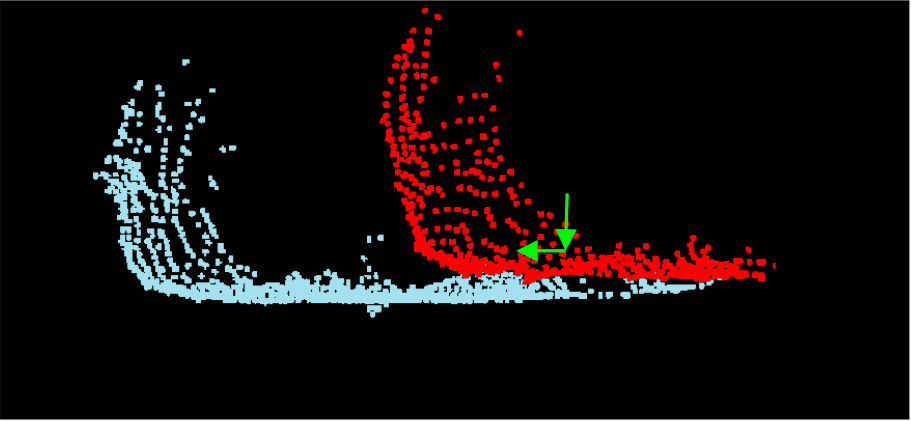
\includegraphics[height=0.25\textwidth]{images/icp-2}};}
    \only<5->{
    \node (program) [outer sep=0,inner sep=0,anchor=south west]
    at (0,0)
    {
    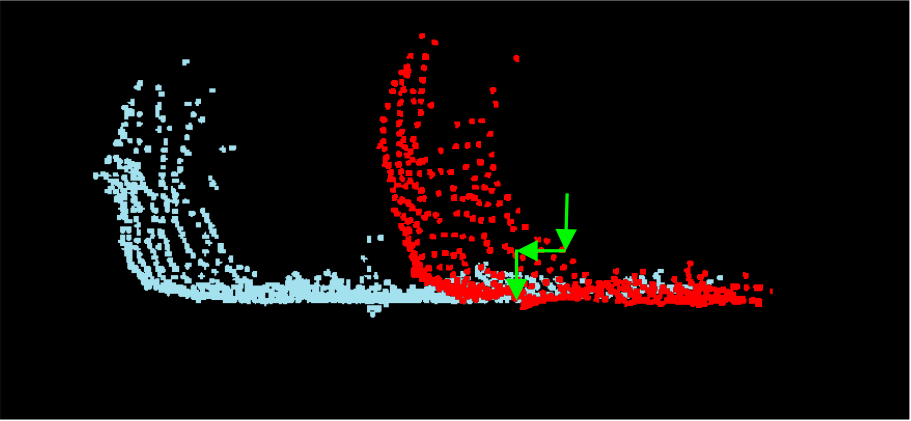
\includegraphics[height=0.25\textwidth]{images/icp-3}};}
    \node (descx) at (5.7,-0.2)
    {\tiny \cite{held-website}};
    \onslide<1->
  \end{tikzpicture}
  \pause
  \pause
  \pause
  \item No motion model
  \end{itemize}
  \end{description}
\end{frame}


\section{Probabilistic Model}

\begin{frame}
  \frametitle{Probabilistic Model}      
  \center
  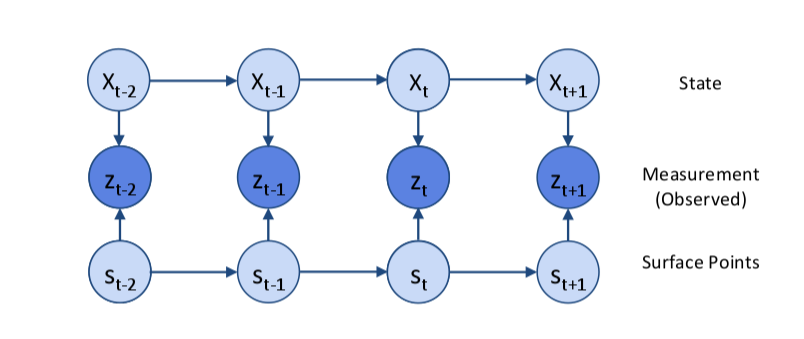
\includegraphics[width=0.8\textwidth]{../img/dbn}
  {\tiny \cite{paper}}
  \begin{description}[]
  \item[Dynamic Bayesian Network] \hfill \\
  \begin{itemize}
  \item Relates variables over successive frames
  \item State $x_t$ (position relative to last frame and velocity)\\
        Surface points $s_t=\{s_{t,1},...,s_{t,n}\}$\\
        Measured point cloud $z_t=\{z_{t,1},...,z_{t,n}\}$
  \item Rotation not considered
  \end{itemize}
  \end{description}
\end{frame}

\begin{frame}
  \frametitle{Probabilistic Model}
  \begin{columns}
  \begin{column}{0.62\textwidth}
  \begin{description}[]
  \item[Surface points] \hfill \\
  \begin{itemize}
  \item Sampled from the visible surface
  \item Indirectly observable
  \item Visible surface varies due to occlusion and viewpoint changes
  \item $p(s_{t,i}|s_{t-1})=p(V)*p(s_{t,i}|s_{t-1},V)+$\\$p(\neg V)*p(s_{t,i}|s_{t-1},\neg V)$
  \item[$\Rightarrow$] $p(s_{t}|s_{t-1}) = \eta(\mathcal{N}(s_t;s_{t-1,i},\Sigma_r) + k)$
  \end{itemize}
  \end{description}
  \end{column}
  \begin{column}{0.4\textwidth}
  \begin{tikzpicture}[thick, every node/.style={font=\footnotesize}]
    \node (program) [outer sep=0,inner sep=0,anchor=south west]
    at (0,0)
    {
    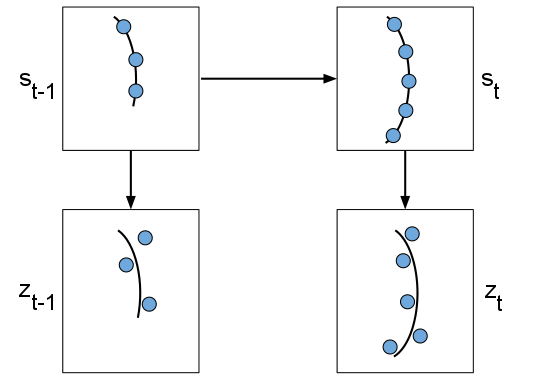
\includegraphics[width=\textwidth]{../img/surface-measurement}};
    \node (descx) at (4.3,-0.2)
    {\tiny \cite{paper}};
  \end{tikzpicture}
  \end{column}
  \end{columns}
\end{frame}

\begin{frame}
  \frametitle{Probabilistic Model}
  \begin{columns}
  \begin{column}{0.62\textwidth}
  \begin{description}[]
  \item[Measurement points] \hfill \\
  \begin{itemize}
  \item Depending on surface points
  \item Gaussian sensor noise $\Sigma_e$
  \item $z_{t,i} \sim \mathcal{N}(s_{t,i},\Sigma_e) + x_{t,p}$\\
        $z_{t-1,i} \sim \mathcal{N}(s_{t-1,i},\Sigma_e)$
  \end{itemize}
  \end{description}
  \end{column}
  \begin{column}{0.4\textwidth}
  \begin{tikzpicture}[thick, every node/.style={font=\footnotesize}]
    \node (program) [outer sep=0,inner sep=0,anchor=south west]
    at (0,0)
    {
    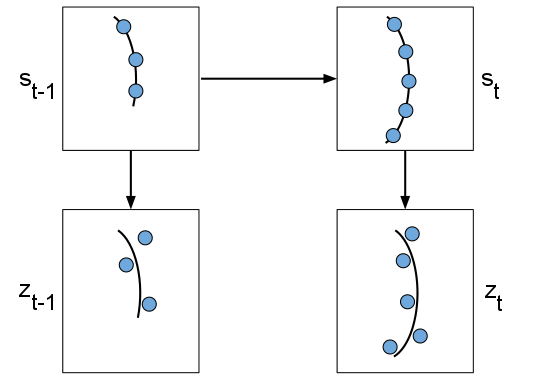
\includegraphics[width=\textwidth]{../img/surface-measurement}};
    \node (descx) at (4.3,-0.2)
    {\tiny \cite{paper}};
  \end{tikzpicture}
  \end{column}
  \end{columns}
\end{frame}

\begin{frame}
  \frametitle{Probabilistic Model}

  \begin{columns}
  \begin{column}{0.4\textwidth}
  \begin{description}[]
  \item[Measurement Model] \hfill \\
  \end{description}
  \end{column}
  \begin{column}{0.6\textwidth}
  \vspace{1cm}
  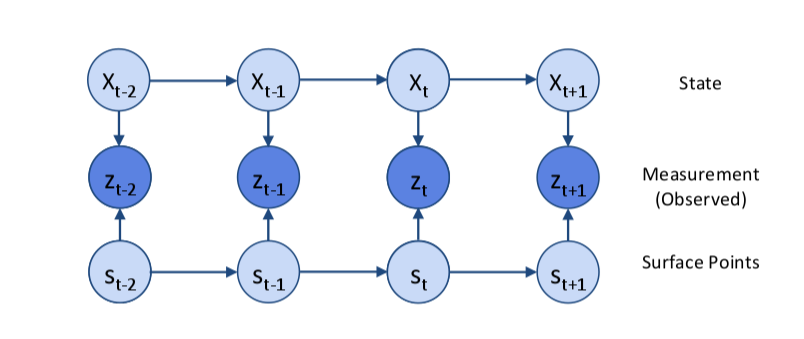
\includegraphics[width=0.9\textwidth]{../img/dbn}
  \end{column}
  \end{columns}
  \vspace{-1cm}
  \begin{align}     
    p(z_t|x_t,z_1,...,z_{t-1}) \onslide<2-> & \approx p(z_t|x_t,z_{t-1}) \nonumber\\
    \onslide<3-> &= \int \int p(z_t,s_t,s_{t-1}|x_t,z_{t-1}) \mathrm d s_t \mathrm d s_{t-1} \nonumber\\
    \onslide<4-> &= \underbrace{\int p(z_t|s_t,x_t) \underbrace{\int p(s_t|s_{t-1})\eta p(z_{t-1}|s_{t-1}) \mathrm d s_t}_{\text{convolution}} \mathrm d s_{t-1}}_{\text{convolution}} \nonumber\\
    \onslide<5-> &= \eta(\mathcal{N}(z_t;z_{t-1}+x_{t,p},\Sigma_r+2\Sigma_e)+k) \nonumber
    \onslide<1->
  \end{align}
\end{frame}

\newcommand{\unaryminus}{\scalebox{0.75}[1.0]{\( - \)}}

\begin{frame}
  \frametitle{Probabilistic Model}
  \begin{description}[]
  \item[Measurement Model Computation] \hfill \\
  \begin{itemize}
  \item $ccp(z_{t,i})$: closest corresponcence point in $z_{t-1}+x_{t,p}$
  \pause
  \item Covariance matrix $\Sigma = 2\Sigma_e+\Sigma_r$
  %say: sigma r funciton of distance
  \pause
  \item Normalization constant $\eta$
  \item Smoothing factor $k$
  %say: found by training
  \onslide<1->
  \end{itemize}
  \end{description}     
  \begin{block}{Measurement Probability}
  \small
  $$
  p(z_t|x_t,z_{t-1}) =
  \eta\prod\limits_{z_{t,i}\in z_t}
  \mathrm{exp}\left(\unaryminus\frac{1}{2}(z_{t,i}\unaryminus\mathrm{ccp}(z_{t,i}))^T\Sigma^{\unaryminus 1}(z_{t,i}\unaryminus\mathrm{ccp}(z_{t,i}))\right)+k
  \nonumber
  $$
  \end{block}
  %say: exchange z_t z_t-1 smaller set into larger one
  %TODO: picture
\end{frame}

\begin{frame}
  \frametitle{Probabilistic Model}
  \begin{description}[]
  \item[Motion Model] \hfill \\
  \begin{itemize}
  \item Kalman filter with constant velocity model
  \item Measurement step: update with Gaussian distribution\\
        $\mu_t=\sum_i p(x_{t,i}|z_1,...,z_t)x_{t,i}$\\
        $\Sigma_t=\sum_i p(x_{t,i}|z_1,...,z_t) (x_{t,i}-\mu_t)(x_{t,i}-\mu_t)^T$
  \item Update step: apply velocity to position
  \end{itemize}
  \end{description}
\end{frame}

\begin{frame}
  \frametitle{Probabilistic Model}
  \begin{itemize}
  \item Dynamic Bayesian Network
  \item Surface points - Measurement points
  \item Derivation of measurement model
  \item Color model
  \item Motion model
  \end{itemize}
\end{frame}

\section{Searching the State Space}
\begin{frame}
  \frametitle{Searching the State Space}
  \begin{itemize}
  \item Dynamic histogram
  \item Refinement step
  \item Annealing
  \end{itemize}
\end{frame}

\section{Evaluation}
\begin{frame}
  \frametitle{Evaluation}
  \begin{itemize}
  \item Videos from website
  \item Relative reference frame approach
  \item Comparison with Kalman and ICP variants
  \item Comparison ADH - densly sampling
  \item Model Crispness approach
  \item Provided Code, experiments
  \end{itemize}
\end{frame}

\section{Conclusion}
\begin{frame}
  \frametitle{Conclusion}
  \begin{itemize}
  \item Catch Phrase
  \item Main Points
  \end{itemize}
\end{frame}



\backupbegin

\begin{frame}[allowframebreaks]
  \frametitle{References}
  %% \nocite{*}
  \bibliographystyle{splncs}
  \bibliography{references}
\end{frame}

\begin{frame}
  \frametitle{Missing stuff}
  \begin{itemize}
  \item related work: alternative sensors, grid-based methods
  \end{itemize}
\end{frame}

\backupend

\end{document}
